\chapter{Design}
\label{chp:design}
This chapter will describe the design process of the administration system.\\
Seeing as the work from previous years will not continue in this project the opportunity to make a new design philosophy rose. 
In 2012 the Launcher group made a design guide. This guide was extended in the Design committee \ref{sub:designGuidelines} and this project will follow that guide. Basically it says that one should follow the colour theme, which can be found in appendix \ref{chap:colorTheme}, and use vector graphics as much as possible. \\
Looking at other web administration interfaces like WordPress \citep{wordpress} the general idea of having a navigation bar at the left side of the screen and the content for a given menu on the right side as figure \ref{fig:ideaWep} shows. This idea also came from the Android systems settings app, which looks like WordPress' admin interface but include a more neutral way of displaying categories. The login page, which is the only page that does not follow the general idea, is inspired directly from Twitter's Bootstrap \citep{bootstrap} sign in layout.\\ 
Every menu-item went through the process of using a whiteboard as a screen and then draw the design by hand. For better preservation, the hand-drawm mockups were created digitally in Balsamiq Mockups \citep{balsamiq}. Next at a meeting showed to our contact person and changed to reflect the issues risen by her. Minutes of the meeting can be found in appendix \ref{interviewMette}. The complete set of final mockups are available in appendix \ref{apx:mockups}.\\

\begin{figure}[!h]
\centering
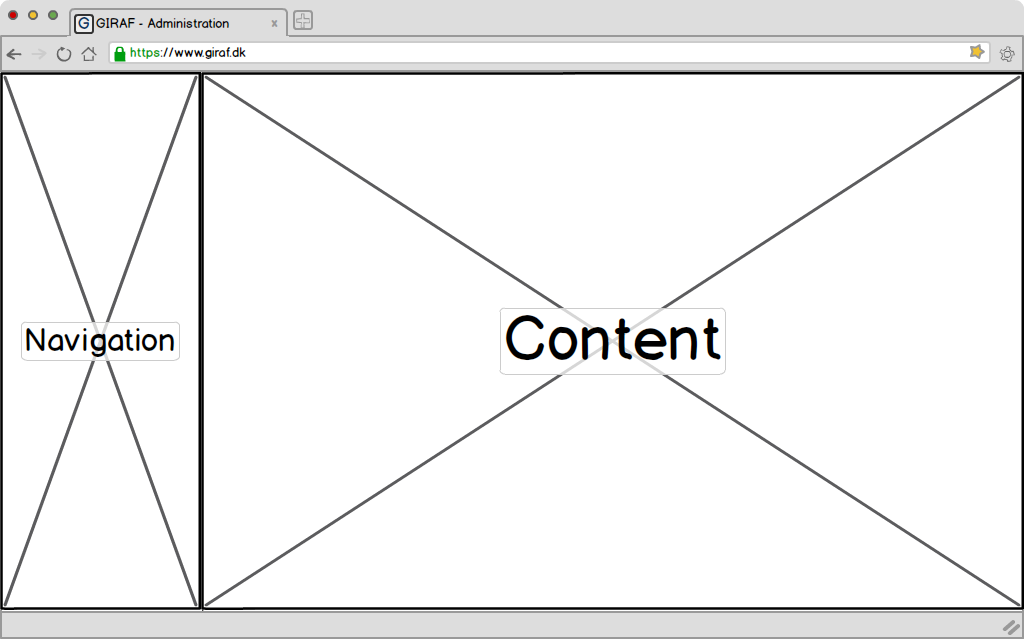
\includegraphics[width=1\textwidth]{images/mockup/displayMode.png}
\caption{General idea of building web-pages.}
\label{fig:ideaWep}
\end{figure}


\section{Designing individual pages}
\subsection{Login}
The Login page is designed to be as minimal as possible. There should be no cluttered information and with a single exception no other option than to login. The exception is to change language. The mockup is viewable in figure \ref{fig:loginDesign}.
\begin{figure}[p]
\centering
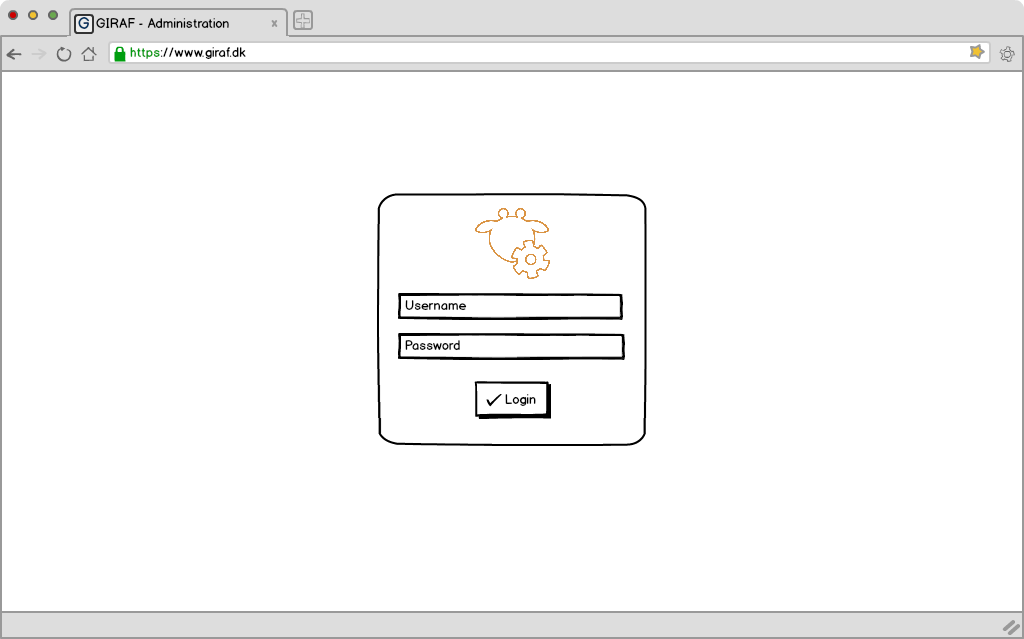
\includegraphics[width=1\textwidth]{images/mockup/login.png}
\caption{Login}
\label{fig:loginDesign}
\end{figure}

\subsection{Navigation}
Navigation was one of the design items that went through a lot of small changes. The general idea was that it should look and feel natural to an Android user. Meaning that the navigation bar conforms to a principle about accessibility so that there are no foldout points or other elements that would be considered difficult to go to on a touch screen. On the mockups each menu category has a little image next to it, this is changed so that now the first letter is capitalized and uses a bigger font than the rest of the text. If a user with administrator rights login he will be able to see all menu items but if a user with degraded rights logs in he will only see Own Profile, Pics Manager and App Manager further information about department as an example is then accessible through own profile without editing rights. A mockup showing the navigation and the profile page is figure \ref{fig:own_profileDesign}.
\begin{figure}[p]
\centering
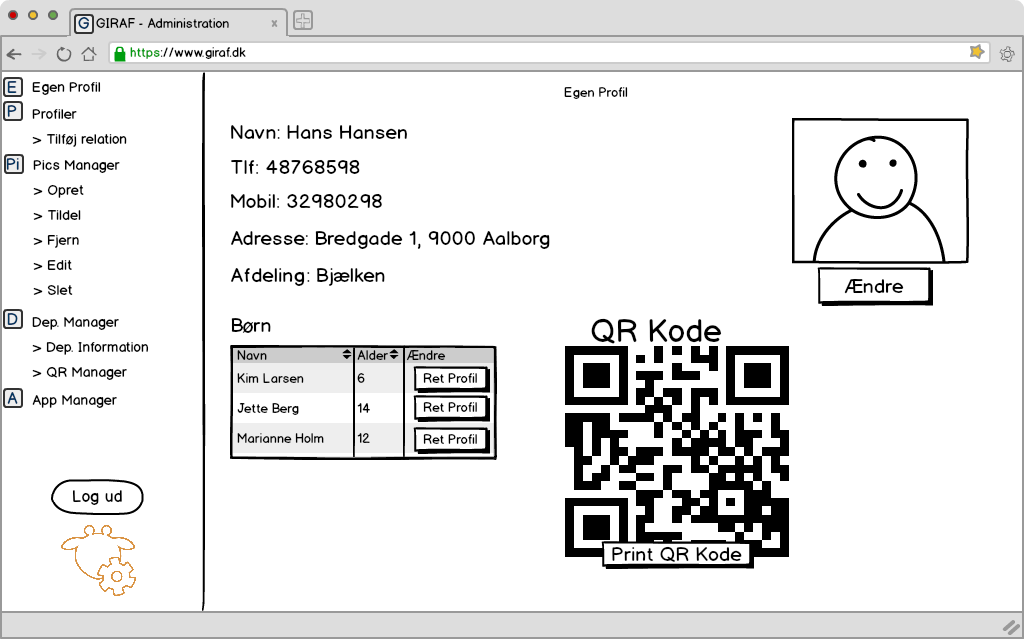
\includegraphics[width=1\textwidth]{images/mockup/egenProfil.png}
\caption{Navigation and Profile page}
\label{fig:own_profileDesign}
\end{figure}

\subsection{Profile Page}
The profile page is the page that is shown when a user logs in. It should have information about the user as well as information about linked profiles such as attached children, parents or pedagogues. A user should also be able to edit his own information as well as attached children information. As a result of our usability test, which can be seen in chapter \ref{chap:usabilityTesting}, the current design used, does not include the ability to change ones QR-code. Instead only the designated admin has that ability. A mockup showing the navigation and the profile page before usability testing is figure \ref{fig:own_profileDesign}.

\subsection{Profiles}
It gives the administrator a complete overview of how users are linked. This sometimes gives a better overview and therefore it is designed so that all links between pedagogues, children and their parents are displayed in an easy to comprehend way. To do this we agreed upon a single table approach which gracefully full-fills the comprehension wanted. This is even more underpinned when colour coding is applied to guide the admin. This idea was given to us by our contact person.

\subsubsection*{Create Profile}
The title say everything. The admins are able to create other profiles. The design consists of a number of input fields as well as the option to select which type of user one wants to create.

\subsubsection*{Add relation}
Here a privileged user should be able to create relations or links between other profiles. A scenario would be that a child profile has just been created and it should now be linked to its already created parents. This procedure should take place here.

\subsection{Pics Manager}
Pics Manager is based upon having the capability to create, add, remove, edit and delete pictograms which all are designed to the same principles of easy accessibility as the rest of the system. Pics Manager should not be accessible on tablets. This is mostly due to the fact that separate applications have been developed for its primary purpose. It should instead open these applications and the user should not be bothered by this. The different components design should have the same look and feel as the Android application but take advantage of the fact that they are run on a desktop computer and not a tablet.
\subsubsection*{Create}
Originally named Make this tool should supply the user with the capability to create pictograms in the database.
\subsubsection*{Add}
Add pictograms to users.
\subsubsection*{Remove}
Remove pictograms from users.
\subsubsection*{Edit}
Enables the user to edit pictograms which the user has available.
\subsubsection*{Delete}
If a user own a pictogram he can delete it permanently from the database.

\subsection{Department Manager}
Enables a privileged user to edit department information and view a short list of attached pedagogues.
\subsubsection*{Department Information}
Essentially the same as Department Manager but displays the information as an unprivileged user would see it. An unprivileged user accesses the page through a link on his profile page.
\subsubsection*{QR Manager}
Enables a privileged user to change users QR-codes. This is also one of the pages which have gone through a number of design iterations, as viewable in appendix \ref{apx:mockups} it originally had three sub items but was refined to a single page with a much more comprehensive layout. This enables the user to complete a given task much more easily. A screenshot of the current layout is figure \ref{fig:qrManagerCurrentDesign}

\section{App. Manager}
The app manager, has only gone through the initial design step. This means that the only thing considered was what it was supposed to represent.\\
The app manager should make it possible to enable or disable the use of certain apps within the GIRAF system, as well as look up description of these.

\begin{sidewaysfigure}[htbp]
\centering
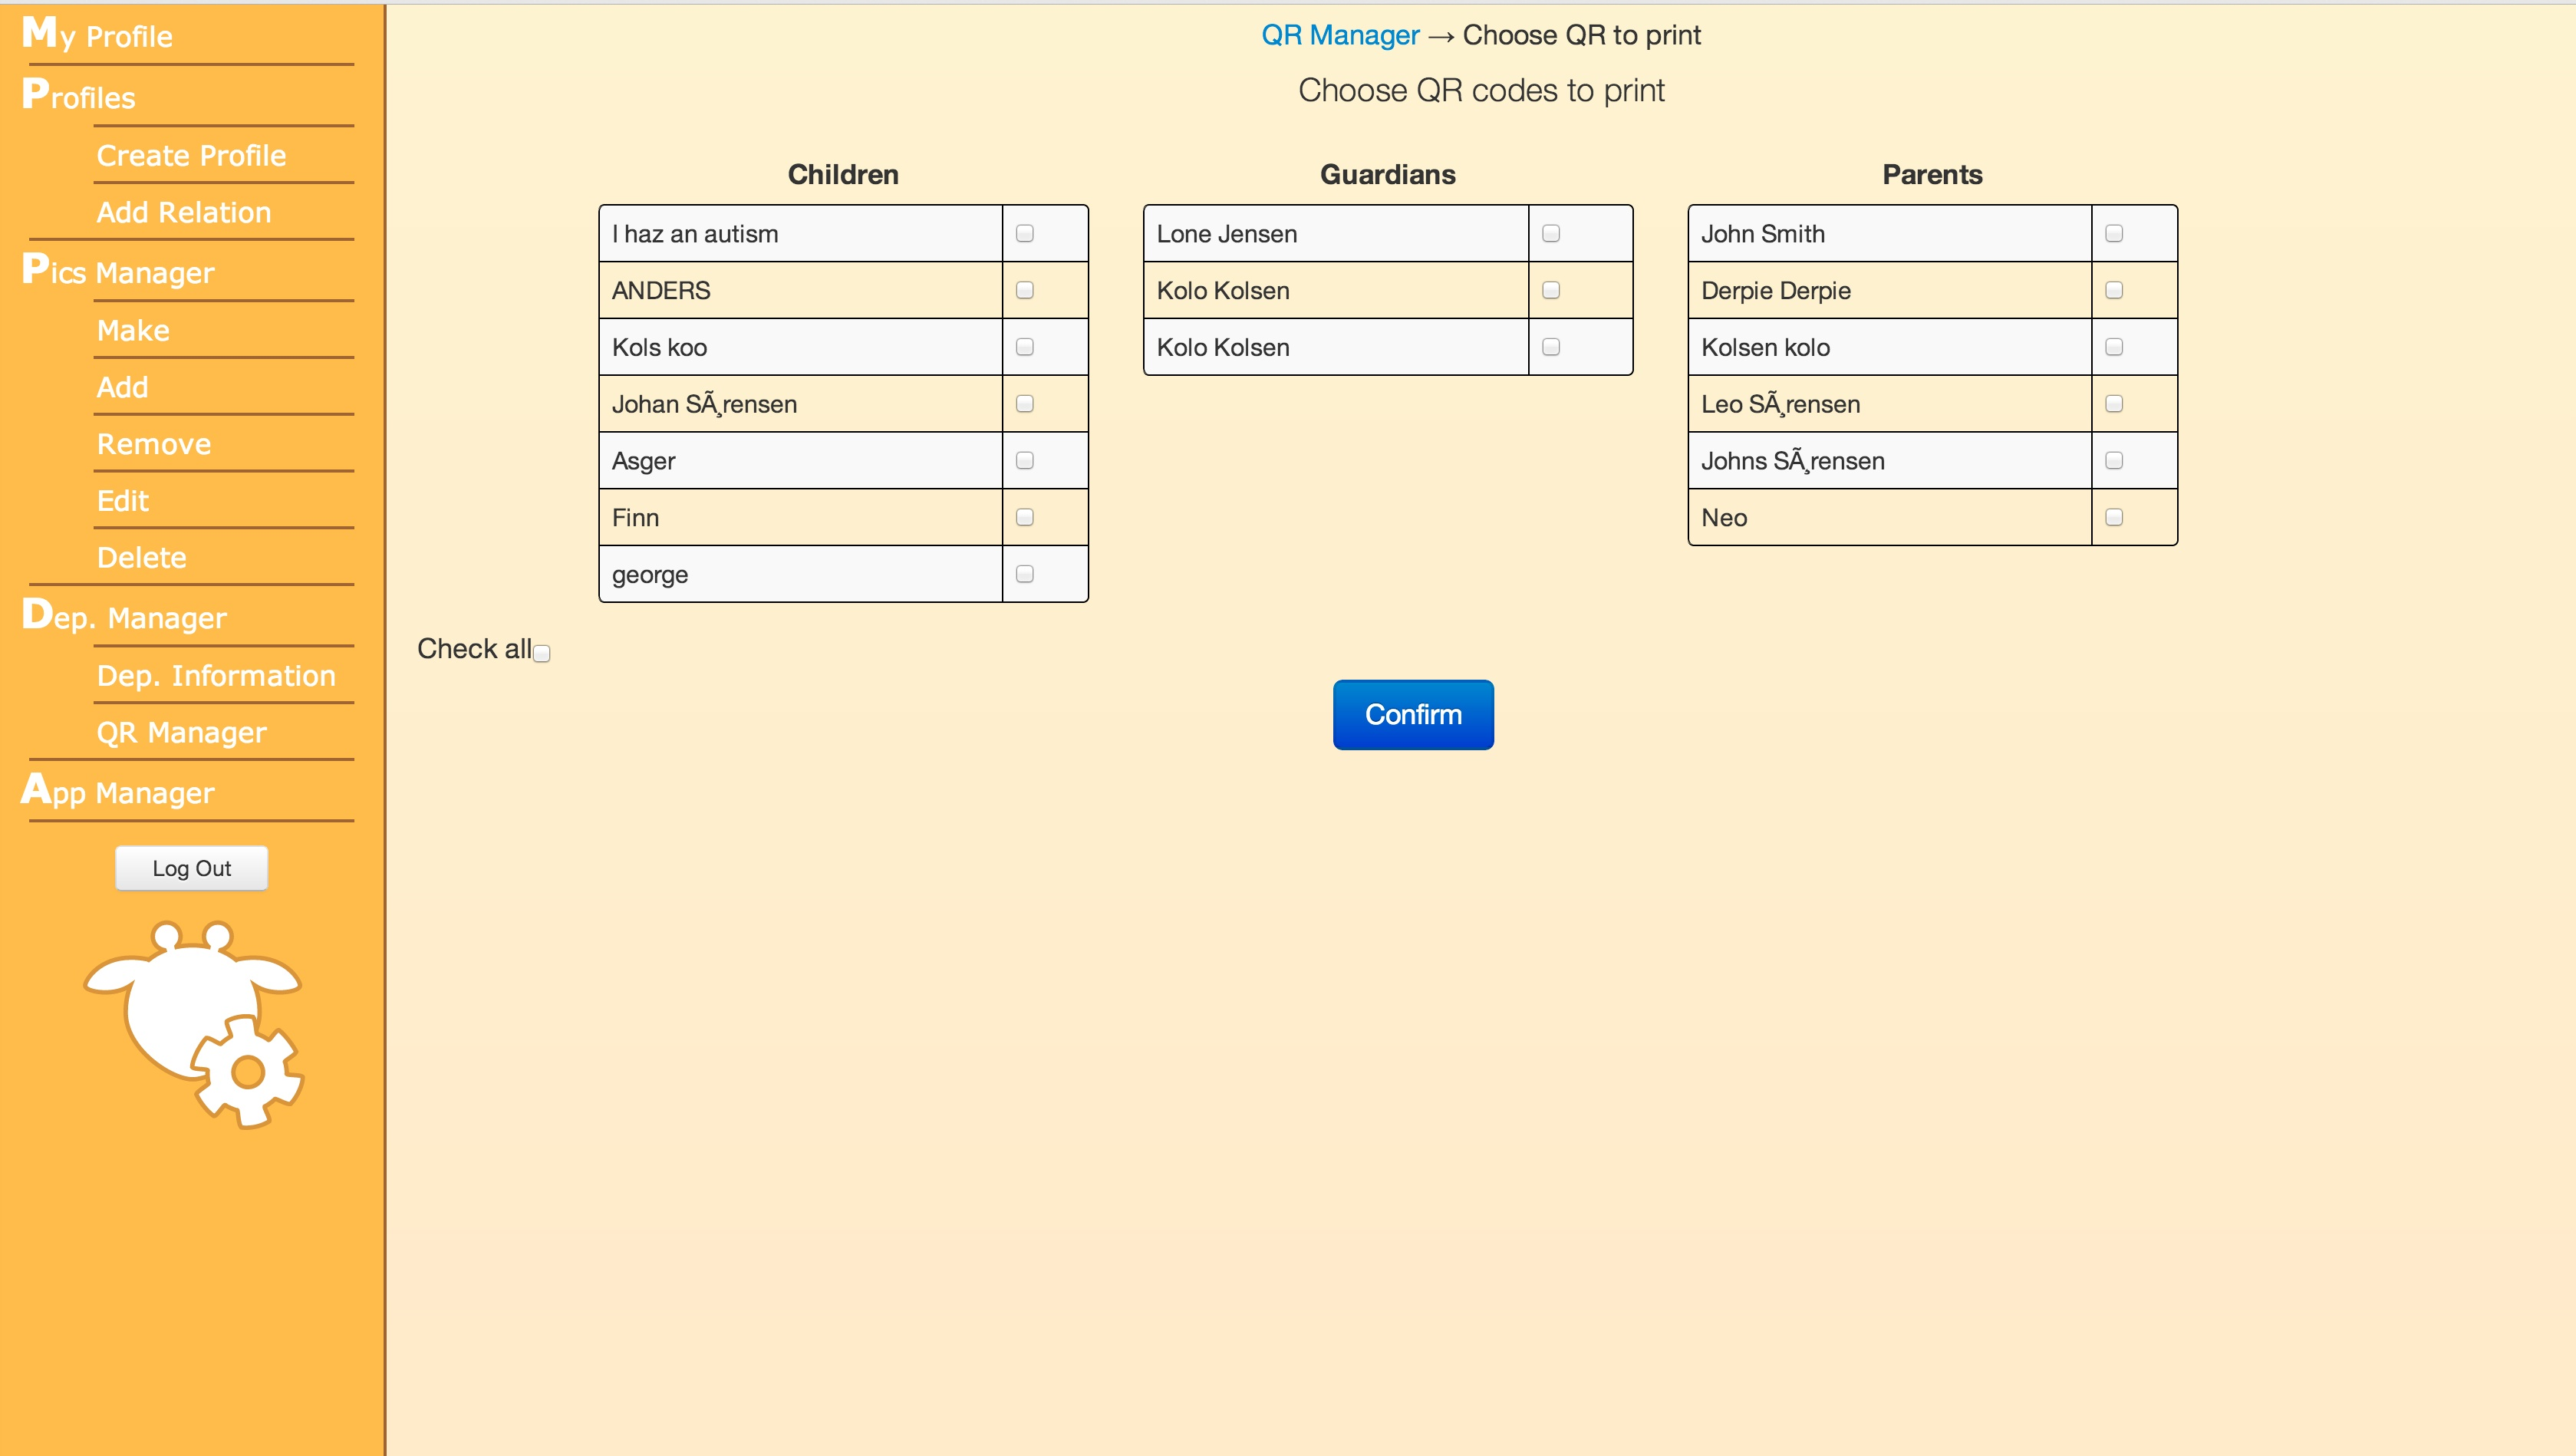
\includegraphics[width=1\textwidth]{images/mockup/qrManagerCurrent.jpg}
\caption{Current design of QR manager}
\label{fig:qrManagerCurrentDesign}
\end{sidewaysfigure}